\chapter{緒論}

\section{研究背景與動機}

近年來,遊戲玩家對於手機遊戲之投入顯得越來越重,尤其是於免付費類型 ( Free-to-Play, F2P ) 之手遊,而非傳統買斷制或月費制類型遊戲。此一商業模式之改變,將使得遊戲商更加注重於遊戲內購買 ( In-App Purchases, IAP ) ,並且在F2P的模式之下,遊戲商之營收有非常顯著的成長,而玩家更加傾向於遊玩F2P類型遊戲,例如:「魔獸世界 ( World of Warcraft )」由於其月費制的商業模式,在2010年至2013年間,因其玩家流失至F2P類型同種遊戲,玩家數大量下滑了30~ \%之多~\cite{drachen2013game};「絕地要塞2 ( Team Fortress 2 )」於2007年為發售買斷制型式遊戲,在2012年改為F2P商業模式,並推出IAP供玩家消費,此一轉變大幅提高遊戲營收達12倍之多~\cite{miller2012gdc}。

因此,如何在F2P類型遊戲中,提高玩家之付費意願,使其透過IAP方式增加遊戲商之營收,顯得格外重要。透過上述情境發想,若能提出一巨量資料探勘框架於遊戲領域,將可以大幅提升預測付費玩家之效率,並且利用預測結果進行玩家消費引導以及了解付費玩家之消費原因與動機。另外,將有助於增加遊戲領域巨量資料探勘之資源,因近幾年來巨量資料研究於遊戲領域呈現下滑狀況~\cite{lee2018game},如圖~\ref{fig:GameDataMiningResearchPaper},於2013年開始便無顯著成長。

\begin{figure}[!htb]
    \begin{center}
      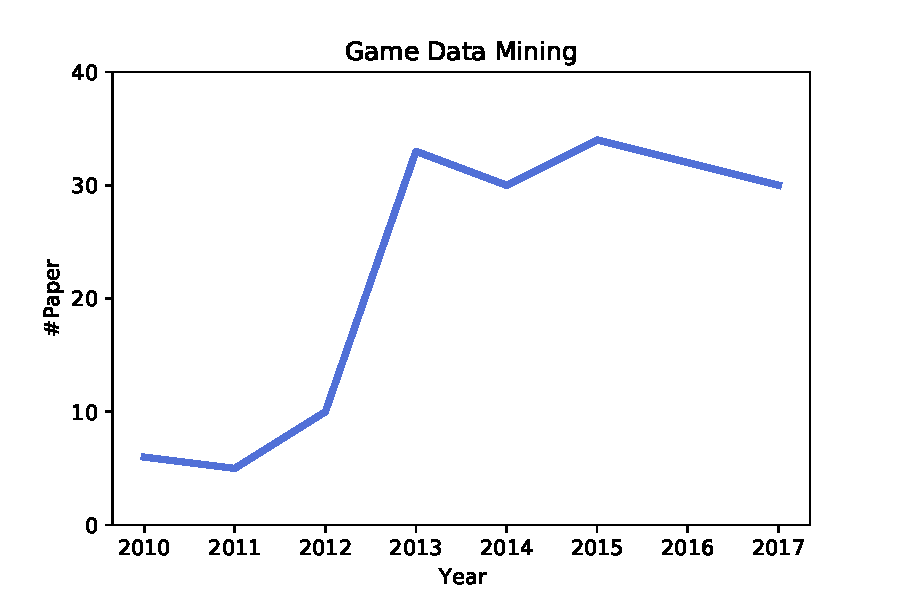
\includegraphics[width=0.7\textwidth]{figures/Image_GameDataMiningResearchPaper.pdf}
      \caption[近年來遊戲領域資料探勘研究數折線圖]{近年來遊戲領域資料探勘研究數折線圖(此圖出自~\cite{lee2018game})}
      \label{fig:GameDataMiningResearchPaper}
    \end{center}
\end{figure}
\newpage

\section{研究目標}

由於提前了解到玩家之付費意願,將有助於遊戲商進行精準行銷於正確的玩家上,使其提升IAP之意願,讓遊戲商可於F2P類型遊戲中獲得良好的營收,又因玩家於進入遊戲初期,將會擁有較高的付費意願。因此,若能藉由一巨量資料探勘框架,來協助遊戲商預測潛在之新進付費玩家,將可減少大量人力成本與時間成本,對於遊戲商有很大的幫助。

本論文的研究目標為預測潛在之新進付費玩家與了解玩家之付費原因。我們將提出一巨量資料探勘框架,包含對於資料集之前處理,並藉由資料分析方法來探索資料之特性,隨後採用機器學習之分類預測,來預測潛在之新進付費玩家,最後依其機器學習預測結果,分析各款遊戲中的突出性,來進行玩家付費原因的解釋說明。

\section{研究方法概述}

本論文對此議題提出一巨量資料探勘框架:此框架將由四大階段組成, (1) 資料前處理階段:首先將從資料庫群中整合所有所需資料,並對其採用直接刪除空缺值樣本方式進行清理,並透過無價值玩家觀察期,刪除無價值玩家資料,以獲取有價值之原始資料,再著手準備目標值與探勘資料特徵,以利後續分析及機器學習使用; (2) 資料分析階段:使用前階段產出之有價值原始資料並透過長條圖與散佈圖來觀察資料特性,進行探索性資料分析 ( Exploratory Data Analysis, EDA ),藉由付費玩家與非付費玩家資料分佈來檢查是否有不合適之資料特徵以及觀察資料特徵是否可以提供給學習模型較多之資訊; (3) 機器學習階段:首先將有價值原始資料集進行分割為訓練及測試集,隨後針對訓練集進行少數群樣本權重值放大以處理不平衡資料與交叉驗證搭配參數表,以獲得最佳模型,其中學習模型選用Decision Tree、Random Forest及Extreme Gradient Boosting,最後藉由測試集來驗證評估最佳模型,產出預測結果; (4) 預測結果分析階段:使用前階段產出之預測結果進行資料特徵重要性分析,透過計算各資料特徵於各學習模型中之$Gini\ Importance$,以利更加了解及解釋資料特徵與遊戲所提供之體驗綜合評估。

在方法驗證上,本論文將藉由$Confusion\ Matrix$所延伸之ROC Curve~\cite{fawcett2006introduction}與PR Curve~\cite{article}來協助驗證學習模型之優劣,並同時利用$Weighted\ F_{beta} - Score$~\cite{Goutte2005API}來選出最佳模型與最佳參數解,隨後計算$Feature\ Importance$於各資料特徵中,以了解到何者於學習模型中貢獻了最多的資訊量,以利學習模型進行訓練與分類。

\section{研究貢獻}

本論文之研究貢獻為:

\begin{enumerate}
    \item 提出一無價值玩家觀察期,可將無價值之玩家資料給予刪除,以利學習模型更加著重於有價值的資訊上。
    \item 提出一付費玩家定義期,可將目標值之準備侷限在新進之玩家上。
    \item 提出一資料特徵探勘期,配合無價值玩家觀察期,以利學習模型更加著重於新進玩家的資訊上。
    \item 於資料集中進行資料特徵之探勘,藉由不同種類與面向之方式,挑選出適合用來呈現付費玩家的資料。
    \item 整理出適合於不平衡資料集中的評估值方式,將對於學習模型之預測結果提供合理的評估,進而進行比較。
    \item 提出一權重值,用於改善資料不平衡之處理,透過將少數群進行放大樣本權重值,使得學習模型更加著重於少數群之資訊。
    \item 整理出資料特徵重要性之計算,以利分析資料特徵的突出性與其貢獻的資訊量。
    \item 提出一巨量資料探勘框架,有效的減少研究時間,並針對各議題進行完善的規劃。
\end{enumerate}

\section{本論文之章節結構}

本論文第~\ref{cha:RelatedWork}~章為文獻探討,針對Free­-to-­Play類型遊戲興起介紹,並探討關於資料前處理、學習模型選擇、資料不平衡處理以及其評估方式的相關文獻。第~\ref{cha:Method}~章為研究方法,詳述講述各階段之研究流程,並分為四節來介紹資料前處理、資料分析、機器學習及預測結果分析。第~\ref{cha:Evaluation}~章為實驗結果與分析,分為五節:第~\ref{sec:SystemStructure}~節 實驗系統架構;第~\ref{sec:DataPreprocessEvaluation}~節 資料前處理評估;第~\ref{sec:DataAnalysisEvaluation}~節 資料分析評估;第~\ref{sec:MachineLearningEvaluation}~節 機器學習評估;第~\ref{sec:PredictionResultAnalysisEvaluation}~節 預測結果分析評估。第~\ref{cha:Conclusions}~章為結論與未來研究,總結本論文提出的方法與實驗結果,並討論未來的研究方向。
\newpage